%%%%%%%%%%%%%%%%%%%%%%%%%%%%%%%%%%%%%%%%%
% Masters/Doctoral Thesis 
% LaTeX Template
% Version 2.5 (27/8/17)
%
% This template was downloaded from:
% http://www.LaTeXTemplates.com
%
% Version 2.x major modifications by:
% Vel (vel@latextemplates.com)
%
% This template is based on a template by:
% Steve Gunn (http://users.ecs.soton.ac.uk/srg/softwaretools/document/templates/)
% Sunil Patel https://www.overleaf.com/3951471463jwsxbnphnkqb?fbclid=IwAR3fUjkfiSBm_HwN_foCwTusuT0JNubmmarfARDr8T7AYkKR33d3CJ-Io7k(http://www.sunilpatel.co.uk/thesis-template/)
%
% Template license:
% CC BY-NC-SA 3.0 (http://creativecommons.org/licenses/by-nc-sa/3.0/)
%
%%%%%%%%%%%%%%%%%%%%%%%%%%%%%%%%%%%%%%%%%

%----------------------------------------------------------------------------------------
%	PACKAGES AND OTHER DOCUMENT CONFIGURATIONS
%----------------------------------------------------------------------------------------

\documentclass[
12pt, % The default document font size, options: 10pt, 11pt, 12pt
oneside, % Two side (alternating margins) for binding by default, uncomment to switch to one side
english, % ngerman for German
onehalfspacing,
%singlespacing, % Single line spacing, alternatives: onehalfspacing or doublespacing
%draft, % Uncomment to enable draft mode (no pictures, no links, overfull hboxes indicated)
nolistspacing, % If the document is onehalfspacing or doublespacing, uncomment this to set spacing in lists to single
%liststotoc, % Uncomment to add the list of figures/tables/etc to the table of contents
%toctotoc, % Uncomment to add the main table of contents to the table of contents
%parskip, % Uncomment to add space between paragraphs
%nohyperref, % Uncomment to not load the hyperref package
headsepline, % Uncomment to get a line under the header
%chapterinoneline, % Uncomment to place the chapter title next to the number on one line
%consistentlayout, % Uncomment to change the layout of the declaration, abstract and acknowledgements pages to match the default layout
]{MastersDoctoralThesis} % The class file specifying the document structureThe class file specifying the document structure

\usepackage[utf8]{vietnam}
\usepackage[utf8]{inputenc} % Required for inputting international characters
\usepackage[T1, T5]{fontenc} % Output font encoding for international characters
\usepackage{mathpazo} % Use the Palatino font by default

\usepackage{amsmath}
\DeclareMathOperator*{\argmax}{arg\,max}
\DeclareMathOperator*{\argmin}{arg\,min}

\usepackage{graphicx}
\graphicspath{ {./Images/} }
\setcounter{tocdepth}{4}
\setcounter{secnumdepth}{4}
\usepackage{commath}
\usepackage{pdfpages}

\usepackage[backend=biber,style=numeric,natbib=true]{biblatex} % Use the bibtex backend with the authoryear citation style (which resembles APA)

\addbibresource{bibliography.bib} % The filename of the bibliography

\usepackage[autostyle=true]{csquotes} % Required to generate language-dependent quotes in the bibliography
\usepackage{listings}


%----------------------------------------------------------------------------------------
%	MARGIN SETTINGS
%----------------------------------------------------------------------------------------

\geometry{
	paper=a4paper, % Change to letterpaper for US letter
	%inner=2.5cm, % Inner margin
	%outer=3.8cm, % Outer margin
	bindingoffset=.5cm, % Binding offset
	%top=1.5cm, % Top margin
	%bottom=1.5cm, % Bottom margin
	%showframe, % Uncomment to show how the type block is set on the page
	left=3.5cm,
	right=2.0cm,
	bottom=3.5cm,
	bmargin=3.0cm,
	tmargin=3.0cm
}
\renewcommand{\baselinestretch}{1.5}
%----------------------------------------------------------------------------------------
%	THESIS INFORMATION
%----------------------------------------------------------------------------------------

\thesistitle{TÌM HIỂU PHƯƠNG PHÁP HỌC SÂU CHO BÀI TOÁN RAIN REMOVAL} % Your thesis title, this is used in the title and abstract, print it elsewhere with \ttitle
\supervisor{TS. Nguyễn Tấn Trần Minh Khang} % Your supervisor's name, this is used in the title page, print it elsewhere with \supname
\examiner{} % Your examiner's name, this is not currently used anywhere in the template, print it elsewhere with \examname
\degree{Doctor of Philosophy} % Your degree name, this is used in the title page and abstract, print it elsewhere with \degreename
\author{Phạm Thị Hoàng Mai\\Hồ Thái Ngọc}
% Your name, this is used in the title page and abstract, print it elsewhere with \authorname
\addresses{} % Your address, this is not currently used anywhere in the template, print it elsewhere with \addressname

\subject{KHOA CÔNG NGHỆ PHẦM MỀM} % Your subject area, this is not currently used anywhere in the template, print it elsewhere with \subjectname
\keywords{} % Keywords for your thesis, this is not currently used anywhere in the template, print it elsewhere with \keywordnames
\university{\href{http://www.uit.edu.vn}{Trường Đại học Công nghệ Thông tin, Đại học Quốc gia TP.HCM}} % Your university's name and URL, this is used in the title page and abstract, print it elsewhere with \univname
\department{\href{http://cs.uit.edu.vn}{Khoa khoa học máy tính}} % Your department's name and URL, this is used in the title page and abstract, print it elsewhere with \deptname
\group{\href{http://researchgroup.university.com}{Research Group Name}} % Your research group's name and URL, this is used in the title page, print it elsewhere with \groupname
\faculty{\href{http://faculty.university.com}{Faculty Name}} % Your faculty's name and URL, this is used in the title page and abstract, print it elsewhere with \facname

\AtBeginDocument{
\hypersetup{pdftitle=\ttitle} % Set the PDF's title to your title
\hypersetup{pdfauthor=\authorname} % Set the PDF's author to your name
\hypersetup{pdfkeywords=\keywordnames} % Set the PDF's keywords to your keywords
}

\begin{document}

\frontmatter % Use roman page numbering style (i, ii, iii, iv...) for the pre-content pages

\pagestyle{plain} % Default to the plain heading style until the thesis style is called for the body content


%----------------------------------------------------------------------------------------
%	TITLE PAGE
%----------------------------------------------------------------------------------------
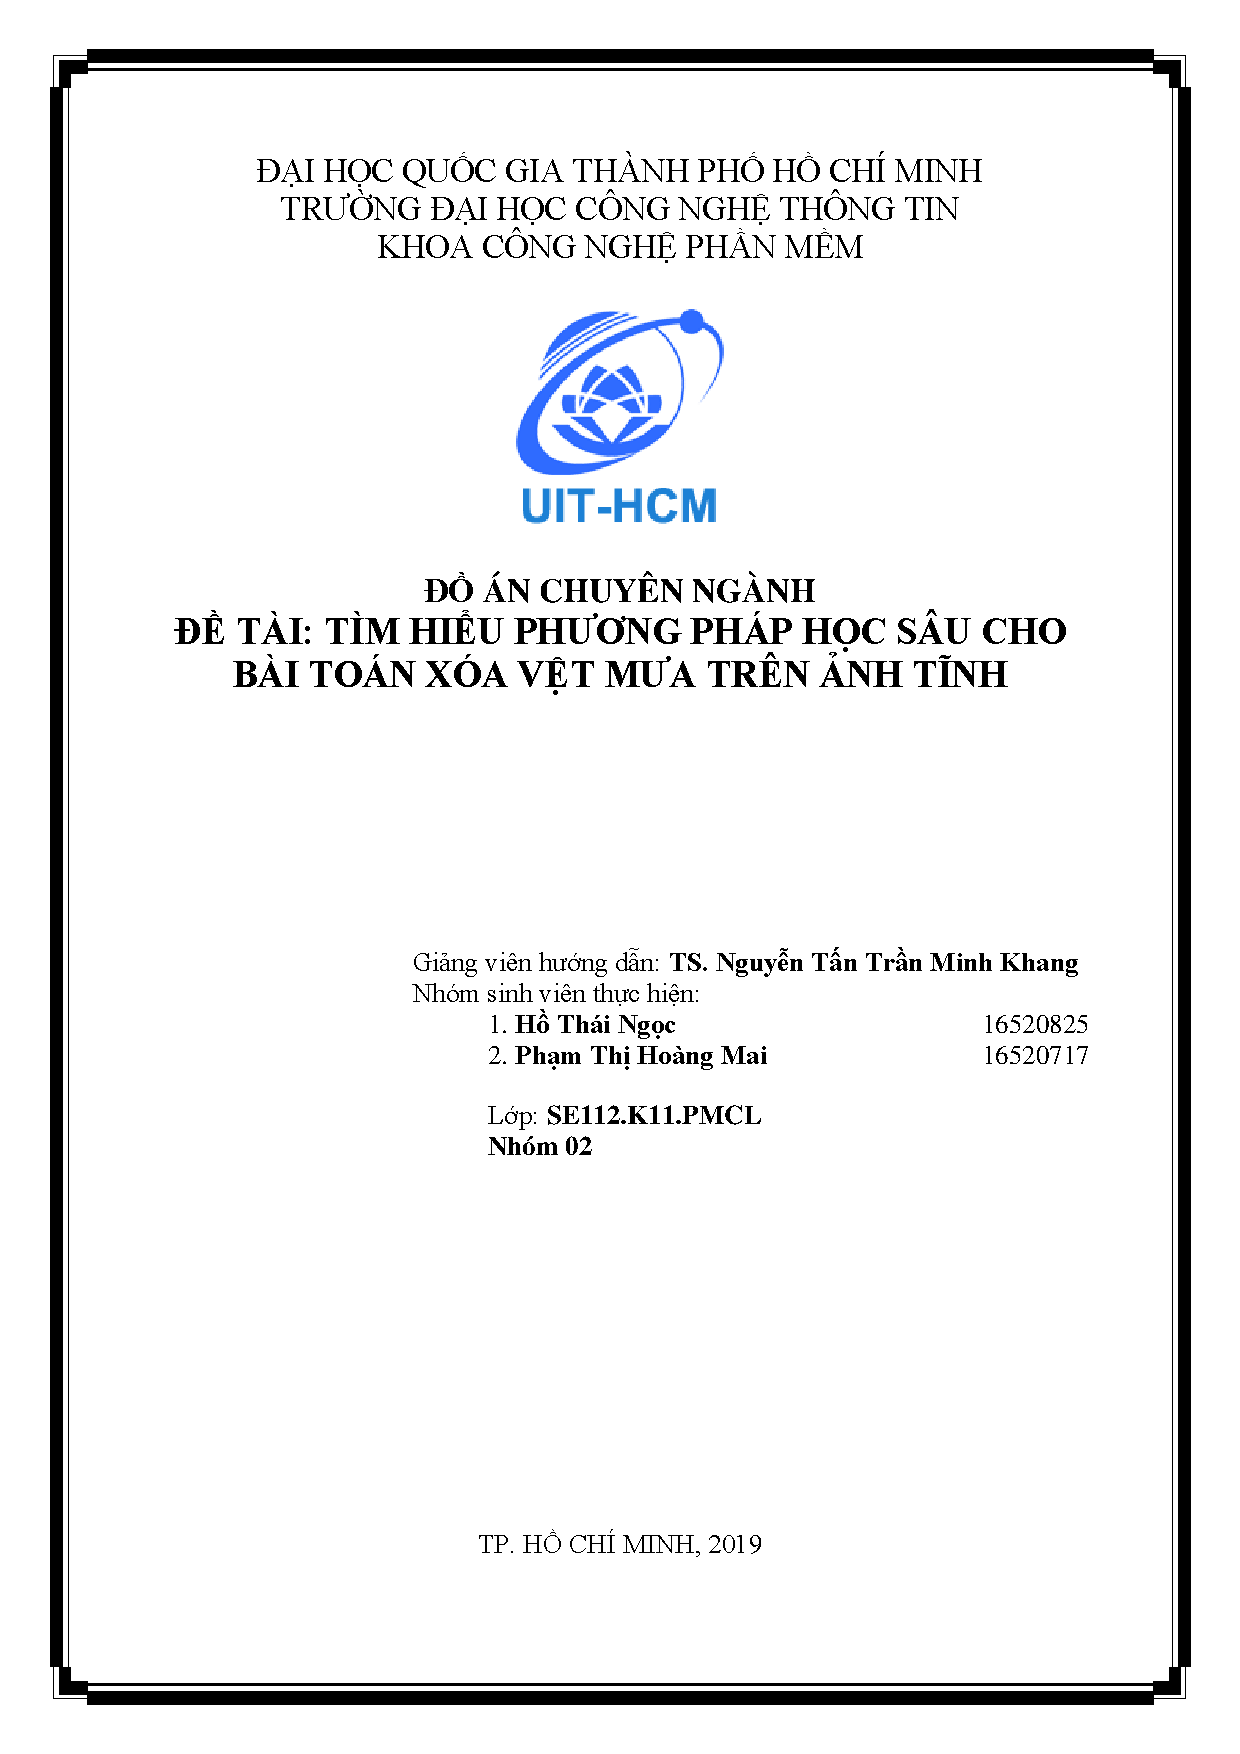
\includepdf[pages=-]{Chapters/Cover/bia_bao_cao_chuyen_nganh_release.pdf}

% \includepdf[pages=-, scale=0.99]{2NHANXET.pdf}

%----------------------------------------------------------------------------------------
%	DECLARATION PAGE
%----------------------------------------------------------------------------------------

% \begin{declaration}
% \addchaptertocentry{\authorshipname} % Add the declaration to the table of contents
% Hội đồng chấm khóa luận tốt nghiệp, thành lập theo Quyết định số ........................
% ngày ....................... của Hiệu trưởng Trường Đại học Công nghệ Thông tin.
% % This prints a line to write the date
% \end{declaration}

\cleardoublepage
\begin{acknowledgements}
% \addchaptertocentry{\acknowledgementname} % Add the acknowledgements to the table of contents
\hspace{10mm}{
Đầu tiên, chúng tôi xin gửi lời cảm ơn chân thành đến tập thể quý thầy cô Trường Đại học Công nghệ thông tin – Đại học Quốc gia TP.HCM và quý thầy cô khoa Công nghệ phần mềm đã giúp cho chúng tôi có những kiến thức cơ bản làm nền tảng để thực hiện nghiên cứu này.
}

\hspace{5mm}{
Đặc biệt, nhóm tác giả xin gửi lời cảm ơn và lòng biết ơn sâu sắc nhất tới TS. Nguyễn Tấn Trần Minh Khang, người thầy đã trực tiếp hướng dẫn, tận tình chỉ bảo và tin tưởng nhóm chúng tôi trong suốt quá trình thực hiện đồ án. Chân thành cảm ơn ThS. Võ Duy Nguyên, phòng thí nghiệm MMLab (UIT) trực thuộc Khoa Khoa học máy tính và Khoa Kỹ
Thuật Thông Tin đã tạo điều kiện về cơ sở vật chất, kỹ thuật, đóng góp nhiều ý kiến quý báu giúp nhóm tác giả hoàn thành tốt đồ án.
}

\hspace{5mm}{
Trong thời gian một học kỳ thực hiện đồ án, nhóm tác giả đã vận dụng những kiến thức nền tảng đã tích lũy đồng thời kết hợp với việc học hỏi và nghiên cứu những kiến thức mới. Từ đó, nhóm tác giả vận dụng tối đa những gì đã thu thập được để hoàn thành một báo cáo đồ án tốt nhất, các kết quả trình bày trong đồ án được tiến hành thực nghiệm trong phòng thí nghiệm MMLab. Tuy nhiên, trong quá trình thực hiện, nhóm tác giả không tránh khỏi những thiếu sót. Chính vì vậy, nhóm tác giả rất mong nhận được những sự góp ý từ phía Thầy Cô nhằm hoàn thiện những kiến thức mà nhóm tác giả đã học tập và là hành trang để nhóm tác giả thực hiện tiếp các đề tài khác trong tương lai.
}
\\
\\
Xin chân thành cảm ơn Thầy Cô.
\hfill
\end{acknowledgements}
%\cleardoublepage

%----------------------------------------------------------------------------------------
%	QUOTATION PAGE
%----------------------------------------------------------------------------------------




%----------------------------------------------------------------------------------------
%	ACKNOWLEDGEMENTS
%----------------------------------------------------------------------------------------


%----------------------------------------------------------------------------------------
%	Mục Lục
%----------------------------------------------------------------------------------------

\tableofcontents % Prints the main table of contents

\listoffigures % Prints the list of figures

\listoftables % Prints the list of tables

%----------------------------------------------------------------------------------------
%	ABBREVIATIONS
%----------------------------------------------------------------------------------------

\begin{abbreviations}{ll} % Include a list of abbreviations (a table of two columns)

\textbf{CNN} & \textbf{C}onvolutional \textbf{N}eural \textbf{N}etwork\\
\textbf{SPANet} & \textbf{SP}atial \textbf{A}ttentive \textbf{N}etwork\\ 
\textbf{IRNN} & Identity Matrix Initialization\\
\textbf{RB} & \textbf{R}esidual \textbf{B}locks \\
\textbf{SAB} & \textbf{S}patial \textbf{A}ttentive \textbf{B}lock\\
\textbf{SARB} &  \textbf{S}patial \textbf{A}ttentive \textbf{R}esidual \textbf{B}lock \\
\textbf{SAM} & \textbf{S}patial \textbf{A}ttentive \textbf{M}odule\\
\textbf{MSE} & \textbf{M}ean - \textbf{S}quare \textbf{E}rror\\
\textbf{PSNR} & \textbf{P}eak \textbf{S}ignal-to- \textbf{N}oise \textbf{R}atio\\
\textbf{SSIM} & \textbf{S}tructural \textbf{S}imilarity \textbf{I}ndex \textbf{M}easure \\


\end{abbreviations}

%----------------------------------------------------------------------------------------
%	ABSTRACT PAGE
%----------------------------------------------------------------------------------------

\begin{abstract}
\addchaptertocentry{\abstractname} % Add the abstract to the table of contents
\hspace{10mm}{
Trong đồ án chuyên ngành này, chúng tôi tập trung nghiên cứu một phương pháp đề xuất được xem là state-of-the-art cho việc giải quyết bài toán Rain removal (loại bỏ mưa trên ảnh tĩnh). Đây là phương pháp đã được được công bố tại hội nghị CVPR - 2019 với mạng học sâu SPatial Attentive Network (SPANet).
}

\hspace{5mm}{
Mục tiêu của đồ án là nghiên cứu về ý tưởng, kỹ thuật cốt lõi cũng như thực nghiệm nó trên bộ dữ liệu đã được tác giả của phương pháp công bố và đồng thời thử nghiệm hiệu suất trên dữ liệu ngẫu nhiên. Qua đó chúng tôi đánh giá kết quả thực nghiệm, phân tích thách thức và đề xuất hướng giải quyết trong tương lai.
}



\end{abstract}
\clearpage





%----------------------------------------------------------------------------------------
%	THESIS CONTENT - CHAPTERS
%----------------------------------------------------------------------------------------

\mainmatter % Begin numeric (1,2,3...) page numbering

\pagestyle{thesis} % Return the page headers back to the "thesis" style

% Include the chapters of the thesis as separate files from the Chapters folder
% Uncomment the lines as you write the chapters
% Sửa lại giới thiệu bài toán, "tạo" ảnh, ảnh input, thách thức,
% Chapter 1

\chapter{Tổng quan} % Main chapter title

\label{Chapter1} % For referencing the chapter elsewhere, use \ref{Chapter1} 

%----------------------------------------------------------------------------------------

% Define some commands to keep the formatting separated from the content 
\newcommand{\keyword}[1]{\textbf{#1}}
\newcommand{\tabhead}[1]{\textbf{#1}}
\newcommand{\code}[1]{\texttt{#1}}
\newcommand{\file}[1]{\texttt{\bfseries#1}}
\newcommand{\option}[1]{\texttt{\itshape#1}}

%----------------------------------------------------------------------------------------

\section{Giới thiệu đề tài}
\subsection{Tổng quan}
\hspace{10mm}{
Chụp ảnh là một cách để ghi lại những giây phút mà chúng ta muốn lưu giữ, những hình ảnh sống động đó sẽ kể lại cả một kỉ niệm, cả một câu chuyên, một quá trình cho người nhìn vào nó.
Những khoảnh khắc xinh đẹp, bùng cháy, những hình ảnh chớp nhoáng, những giây phút bên nhau... đều được ghi lại một cách chân thực nhất trong những tấm hình.}

\hspace{5mm}{
Một hình ảnh được chụp kèm theo các yếu tố không mong đợi như vệt mưa, hạt mưa, sương mù... Hiển nhiên rằng, chúng sẽ gây cản trở nghiêm trọng đến khả năng quan sát các vật thể trong ảnh cũng như là giá trị thực sự của khoảnh khắc mà bức ảnh muốn lưu lại.
}

\hspace{5mm}{Trong những năm gần đây, giới nghiên cứu đang chứng kiến sự tiến bộ đáng kể trong việc xoá bỏ các yếu tố gây cản trở tầm nhìn trên một bức ảnh. Sự phát triển của lĩnh vực này chung quy lại chính là do sự phát triển của nhiều thuật toán và phương pháp ứng dụng các mô hình học sâu dựa trên mạng neural tích chập (CNNs). Đây chính là một trong những chìa khóa mang theo sứ mệnh kết nối hình ảnh và khoảnh khắc trọn vẹn.}

\subsection{Giới thiệu bài toán} 
\hspace{10mm}{Single image deraining là bài toán có mục tiêu là loại bỏ các yếu tố cản trở vật thể trên ảnh, mà cụ thể ở đây là mưa. Bài toán Single image deraining có đầu vào là một bức ảnh có mưa và đầu ra là ảnh đã được xoá bỏ mưa (Hình \ref{fig:gioi-thieu-bai-toan}).\\} 

\begin{figure}[ht!]
    \includegraphics[width=\textwidth]{Images/Chapter-3/img-Ch3-mua-gt-362.png}
    \caption{(a) Ảnh không mưa,  (b) Ảnh có mưa}
    \label{fig:gioi-thieu-bai-toan}
\end{figure}
\subsection{Đối tượng nghiên cứu}
\hspace{10mm}{Hình ảnh có tầm nhìn bị ảnh hưởng do các yếu tố ngoại cảnh. Trong đồ án này, mưa là đối tượng được nhóm tác giả nghiên cứu. Hiện nay, mưa được chia thành 3 loại chính (\ref{fig:rain}):}
\begin{itemize}
    \item Giọt mưa
    \item Vệt mưa
    \item Mưa và sương mù
\end{itemize}
\begin{figure}[h]
    \centering
    \includegraphics[width=15cm]{Images/Chapter-1/rain.png}
    \caption{(a) Giọt mưa, (b) Vệt mưa, (c) Mưa và sương mù.}
    \label{fig:rain}
\end{figure}
\section{Thách thức của bài toán và giải pháp đã công bố}
\subsection{Thách thức}
\begin{itemize}
    \item Đầu tiên, các bộ dữ liệu tổng hợp hình ảnh mưa hiện có:  Multi-Purpose Image Deraining (MPID) \cite{Li2019DerainBenchmark},... vẫn còn nhiều hạn chế về mặt thực tế. Các bộ dữ liệu thường được tạo ra từ một tấm ảnh bình thường sau đó thêm hạt mưa vào ảnh ban đầu. Tuy nhiên, phương pháp này vẫn chưa thể mô hình hoá các đặc điểm vật lý của giọt mưa trong tự nhiên như hình dạng, hướng và cường độ mưa.
    \item Thứ hai, các nhà nghiên cứu chủ yếu đánh giá hiệu suất dựa trên việc so sánh trực quan với hình ảnh thực tế. Điều này khiến cho việc đánh giá bớt khách quan đi.
    \item Thách thức cốt lõi nhất trong việc đề xuất cách tổ chức dữ liệu dưới dạng tập hợp các cặp ảnh (ảnh mưa/ ảnh không mưa) đó là hai loại ảnh này không thể tạo ra trong cùng một thời điểm, đó là do tính chất ngẫu nhiên của mưa và giới hạn về thời gian thực của các kỹ thuật tạo ảnh.
\end{itemize}
\subsection{Giải pháp đã được công bố}
\hspace{10mm}{Cho đến thời điểm hiện tại việc nghiên cứu giải pháp giải quyết vấn đề xóa yếu tố mưa trên ảnh cũng đạt nhiều thành tựu đáng kể. Nhiều phương pháp, thuật toán đã được công bố tại các hội nghị về thị giác máy tính. Tuy nhiên, các thuật toán này chủ yếu được đánh giá bằng cách sử dụng một số loại hình ảnh tổng hợp nhất định, giả sử một mô hình mưa cụ thể, cộng với một vài hình ảnh thực. Do đó, không rõ các thuật toán này sẽ hoạt động như thế nào trên các hình ảnh mưa thu được trong thế giới thật và cách chúng ta có thể đánh giá tiến trình trong lĩnh vực này.}

\hspace{5mm}{
Dưới đây là sáu phương pháp hoặc đề xuất được xem là state-of-the-art trong lĩnh vực xóa mưa trên ảnh tĩnh, áp dụng trên bộ dữ liệu Multi-Purpose Image Deraining (MPID) \cite{Li2019DerainBenchmark}.
}

\begin{itemize}
    \item Gaussian mixture models (GMMs) \cite{li2016rain}
    \item JOint Rain DEtection and Removal (JORDER) \cite{yang2017deep}
    \item Deep Detail Network (DDN) \cite{fu2017removing}
    \item Conditional Generative Adversarial Network (CGAN) \cite{zhang2019image}
    \item Density-aware Image Deraining method using a Multistream Dense Network (DIDMDN) \cite{zhang2018density}
    \item DeRaindrop \cite{qian2018attentive}
\end{itemize}

\begin{table}[h!]
\centering
\begin{tabular}{|l|c|c|c|c|c|c|}
\hline
 & \multicolumn{1}{l|}{Degraded} & \multicolumn{1}{l|}{GMM} & \multicolumn{1}{l|}{JORDER} & \multicolumn{1}{l|}{DDN} & \multicolumn{1}{l|}{CGAN} & \multicolumn{1}{l|}{DID-MDN} \\ \hline
\multicolumn{7}{|c|}{rain streak} \\ \hline
\textbf{PSNR} & 25.95 & 26.88 & 26.26 & \textbf{29.39} & 21.86 & 26.80 \\ \hline
\textbf{SSIM} & 0.7565 & 0.7674 & \textbf{0.8089} & 0.7854 & 0.6277 & 0.8028 \\ \hline
\end{tabular}
\caption[Bảng thông kê hiệu suất các phương pháp đề xuất]{Đánh giá hiệu suất dựa trên độ đo PSNR, SSIM \cite{Li2019DerainBenchmark} \cite{hore2010image}}
\label{tab:danh-gia-1}
\end{table}

%----------------------------------------------------------------------------------------
\section{Mục tiêu, đóng góp}
\subsection{Mục tiêu}
\begin{itemize}
    \item Hiểu được pipeline cơ bản của tiến trình xoá mưa trên ảnh đơn (single image deraining)
    \item Nắm bắt ý tưởng, kỹ thuật cơ sở của state-of-the-art SPANet.
    \item Cài đặt và thực nghiệm phương pháp đề xuất đã tìm hiểu.
    \item Thực nghiệm phương pháp trên các bộ dữ liệu đã được công bố trong lĩnh vực rain removal.
    \item Thu thập kết quả thực nghiệm, đánh giá hiệu suất, thách thức của phương pháp, đưa ra đề xuất phát triển.
\end{itemize}

\subsection{Đóng góp}
\begin{itemize}
    \item Tìm hiểu và thực nghiệm phương pháp đề xuất bán tự động kết hợp các đặc tính tạm thời của mưa cùng với sự giám sát của con người để xây dựng một bộ dữ liệu mưa thật quy mô lớn.
    \item Thực nghiệm trên bộ dữ liệu khoảng 29.5K ảnh, gồm tập hợp các cặp ảnh đối chiếu tương phản (ảnh mưa tự nhiên có độ phân giải cao/ ảnh không mưa). Cách tổ chức dữ liệu này giúp cải thiện hiệu suất cho các phương pháp state-of-the-art trong bài toán xóa mưa trên ảnh tĩnh.
    \item Nghiên cứu kiến trúc mạng SPatial Attentive Network (SPANet) một đề xuất state-of-the-art ở hội nghị CVPR - 2019 nhằm giải quyết bài toán loại bỏ vệt mưa trên ảnh.
    \item Ứng dụng hai độ đo Peak signal-to-noise ratio (PSNR) và Structural similarity index measure (SSIM) đánh giá kết quả thực nghiệm từ kiến trúc SPANet.
\end{itemize}

\clearpage
\section{Nội dung đồ án chuyên ngành}
\begin{itemize}
    \item Cái nhìn tổng quan về phương pháp học sâu, tiềm năng ứng dụng trong nghiên cứu và thực nghiệm.
    \item Tìm hiểu cách giải quyết bài toán xoá mưa trên ảnh đơn (single image deraining).
    \item Nghiên cứu về state-of-the-art Spatial Attentive Single-Image Deraining \cite{wang2019spatial}.
    \item Qui trình cài đặt, thực nghiệm phương pháp trên bộ dữ liệu tương ứng.
    \item Kết luận, đánh giá kết quả đạt được, nêu hạn chế, định hướng phát triển.
\end{itemize}

\section{Cấu trúc đồ án}
\hspace{10mm}{Phần còn lại của khóa luận được tổ chức như sau: Ở chương 2 chúng tôi sẽ trình bày các cơ sở lý thuyết phục vụ cho bài toán và trình bày chi tiết các phần quan trọng trong state-of-the-art Spatial Attentive Network. Chương 3 chúng tôi sẽ trình bày môi trường và cách thức chạy thực nghiệm, kết quả đánh giá hiệu suất và nhận xét. Chương 4 đưa ra kết luận và tổng kết về những gì đạt được, cùng với đó là đề ra các hướng nghiên cứu trong tương lai.}
% Chapter 1

\chapter{Cơ sở lý thuyết} % Main chapter title

\label{Chapter2} % For referencing the chapter elsewhere, use \ref{Chapter1} 

%----------------------------------------------------------------------------------------

% Define some commands to keep the formatting separated from the content 


%----------------------------------------------------------------------------------------
\section{Machine Learning và Deep Learning}
\hspace{10mm}{
Trí tuệ nhân tạo trong nhiều thập kỷ qua là mô hình máy tính có khả năng học, suy nghĩ và ra quyết định giống như con người. Trước khi học máy xuất hiện, việc tính toán dựa trên kinh nghiệm nhiều hơn là sử dụng các chương trình trên nền tảng các qui luật. Từ khi xuất hiện, trí tuệ nhân tạo đã phát triển mạnh mẽ và trở thành nền tảng cho cách mạng công nghiệp 4.0.}

\hspace{5mm}{
Deep Learning có thể xem là một nhánh của học máy được phát triển và trở thành xu hướng mới cho việc cải thiện mạng neural trong vấn đề về chi phí và độ chính xác. Thuận ngữ "Deep" trong Deep Learning đề cập đến khả năng có nhiều phân lớp hơn ở giữa các mạng neural, chính là các lớp ẩn (hidden layers) khi so sánh với kiến trúc ban đầu. Sự cải thiện này cho phép máy tính có khả năng xử lý các tập dữ liệu lớn trong khi các kiến trúc mạng truyền thống thì không đáp ứng được. Nhờ vào Deep Learning, nhiều giải pháp được đưa ra nhằm giải quyết các bài toán học máy một cách dễ dàng với độ chính xác cao, góp phần đưa trí tuệ nhân tạo phục vụ nhu cầu cuộc sống của con người trên nhiều khía cạnh.}

\hspace{5mm}{
Những nhân tố góp phần giúp thúc đẩy sự bùng nổ các phương pháp học sâu và giúp chúng trở thành xu hướng mới của thời đại:
\begin{itemize}
    \item Sự ra đời của các bộ dữ liệu lớn được gán nhãn.
    \item Sự ra đời của ReLU và các hàm kích hoạt liên quan làm hạn chế vấn đề vanishing gradient.
    \item Sự cải tiến của các kiến trúc: GoogLeNet, VGG, ResNet, … và các kỹ thuật transfer learning, fine tuning.
    \item Nhiều thư viện mới hỗ trợ việc huấn luyện deep network với GPU: theano, caffe, mxnet, tensorflow, pytorch, keras, …
    \item Khả năng tính toán song song tốc độ cao của GPU.
\end{itemize}
}

\section{Mạng Neural Network}
\hspace{10mm}{
Neural Network là một phát minh quan trọng, góp phần thúc đẩy sự phát triển vượt bậc của công nghệ đặc biệt trong các lĩnh vực về khoa học máy tính. Về cơ bản, mạng neural dùng để rút trích đặc trưng mô hình chung của một bộ dữ liệu đầu vào định sẵn, dựa vào đó các nhà nghiên cứu có thể sử dụng để phân tích thông tin, phát triển các giải pháp giải quyết các vấn đề khác nhau. Kiến trúc căn bản của một mạng neural network là tổ hợp của nhiều lớp (layer) được phân ra ba nhóm chính: lớp đầu vào (Input layer), các lớp ẩn (Hidden layers), lớp đầu ra (Output layer). Hình \ref{fig:neural-network-1} cho thấy, một lớp riêng biệt có nhiều nút điểm, đây là nơi diễn ra các tác vụ chính của lớp. Các nút điểm được nối với nhau thông qua các liên kết sao cho dữ liệu đầu ra của lớp này là đầu vào của lớp kế tiếp, dữ liệu sẽ tiếp tục được xử lý để thu được kết quả mong muốn ở lớp cuối cùng.
}

\begin{figure}[h]
    \centering
    \includegraphics[width=12cm]{Images/Chapter-2/img-mang-neural-network-1.png}
    \caption{Minh họa mạng Neural Network}
    \label{fig:neural-network-1}
\end{figure}
\subsection{Neural nhân tạo (perceptron)}
\hspace{10mm}{
Hình thức cơ bản của mạng neural nhân tạo được đưa ra bởi  Frank Rosenblatt tại phòng thí nghiệm Corell Aeronautical vào những năm 1950. Ông đã đưa ra mô hình bằng cách mô phỏng bộ não con người. Bộ não con người là tập hợp các tế bào thần kinh được cấu thành từ phần thân (soma) với nhân ở bên trong và xung quanh có nhiều sợi nhánh với một sợi trục chính, các tế bào thần kinh kết nối với nhau thông qua sợi nhánh và sợi trục. Các xung động thần kinh được tiếp nhận từ sợi nhánh sẽ được gửi vào phần thân xử lý, xung động lan truyền qua sợi trục, nếu chúng vượt ngưỡng, xung thần kinh được lan truyền cho các tế bào thần kinh khác (Hình \ref{fig:te-bao-than-kinh}).
}
\begin{figure}[h]
    \centering
    \includegraphics[width=12cm]{Images/Chapter-2/img-neuron.png}
    \caption{Tế bào thần kinh sinh học}
    \label{fig:te-bao-than-kinh}
\end{figure}

\hspace{5mm}{
Dựa trên cấu trúc và nguyên lý lan truyền xung thần kinh của bộ não người, neural nhân tạo lấy các giá trị đầu vào \(x_{1}, x_{2}, ..., x_{n}\) từ các neural khác, cùng với \(w_{1}, w_{2}, ..., w_{n}\) đại diện cho tín hiệu đầu ra. Thay thế cho ngưỡng lan truyền xung thần kinh chính là tập các hàm kích hoạt (activation). Hình \ref{fig:te-bao-neural-nhan-tao} cho thấy sự tương đồng giữa kiến trúc neural nhân tạo và tế bào thần kinh sinh học ở người. Bên cạnh đó, đầu ra của một neural nhân tạo thường là giá trị nhị phân, về mặt toán học thì neural có thể được biểu diễn như sau: }
\begin{equation}
f = \left\{\begin{matrix}
1 & if & \sum_{i=1}^{n} w_{i}x_{i} + b_{i} >  0\\ 
0 & if & \sum_{i=1}^{n} w_{i}x_{i} + b_{i} \leq   0
\end{matrix}\right.
\end{equation}

\begin{figure}[h]
    \centering
    \includegraphics[width=12cm]{Images/Chapter-2/img-perceptron.png}
    \caption{Mô hình neural nhân tạo}
    \label{fig:te-bao-neural-nhan-tao}
\end{figure}

\subsection{Mạng neural đa lớp}
\hspace{10mm}{
Xét đến việc giải quyết một vấn đề phức tạp, một vài neural nhân tạo hiển nhiên là chưa đủ, do đó cần phải tổ chức lại các neural thành một cấu trúc mạng thống nhất với quy mô lớn về số lượng neural cũng như là kết cấu phức tạp hơn. Hình \ref{fig:mang-dien-hinh} mô tả kiến trúc mạng điển hình, với một lớp đầu vào theo sau đó là tập \(n\) lớp ẩn liên tục nhận tín hiệu từ lớp trước nó liên kết để tạo thông tin trừu tượng cho lớp tiếp theo. Quá trình này sẽ lặp lại cho đến lớp đầu ra cuối cùng, nơi mà quyết định được đưa ra.
}

\begin{figure}[h]
    \centering
    \includegraphics[width=12cm]{Images/Chapter-2/img-multiple-neural.png}
    \caption{Kiến trúc mạng neural nhân tạo với 3 lớp ẩn}
    \label{fig:mang-dien-hinh}
\end{figure}

\subsection{Hàm kích hoạt (Activation function)}
\begin{figure}[h]
        \centering
        \includegraphics[width=10cm]{Images/Chapter-2/img-dothi-sigmoid.png}
        \caption{Đồ thị hàm Sigmoid}
        \label{fig:dothi-sigmoid}
\end{figure}
\begin{figure}[h]
        \centering
        \includegraphics[width=10cm]{Images/Chapter-2/img-dothi-tanh.png}
        \caption{Đồ thị hàm Tanh}
        \label{fig:dothi-tanh}
\end{figure}
\begin{figure}[h]
        \centering
        \includegraphics[width=14cm]{Images/Chapter-2/img-sosanh-relu.png}
        \caption{So sánh đồ thị Sigmoid và ReLU}
        \label{fig:dothi-relu}
\end{figure}
\begin{figure}[h]
        \centering
        \includegraphics[width=10cm]{Images/Chapter-2/img-dothi-softmax.png}
        \caption{Đồ thị Softmax}
        \label{fig:dothi-softmax}
\end{figure}
\hspace{10mm}{
Trong quá trình học, trọng số và bias được tinh chỉnh dần theo thời gian để đưa kết quả tiến gần đến giá trị thực. Ngoài một hàm mất mát (loss function) được thiết kết để ước tính lỗi và truyền lại tín hiệu cho neural điều chỉnh tham số thì còn có một hàm kích hoạt. Hàm kích hoạt được thiết lập ở mỗi neural với nhiệm vụ ánh xạ đầu ra từ neural đến miền giá trị mong muốn trước khi lan truyền kết quả ấy đến những neural khác đảm bảo duy trì việc học của mạng được tiếp diễn. Hàm kích hoạt phải là hàm phi tuyến tính để dữ liệu đầu ra cũng có tính chất phi tuyến, đều này rất quan trọng nếu không muốn phá vỡ phân cấp kiến trúc mạng và biến đổi nó thành một tổ hợp tuyến tính.
}
\begin{itemize}
    \item Hàm sigmoid (Hình \ref{fig:dothi-sigmoid}): Đây là hàm được sử dụng phổ biến vì độ phức tạp thấp, mô phỏng tốc độ neural sinh học và đưa các giá trị về miền [0,1]. Tuy nhiên, hàm kích hoạt này sẽ bị giới hạn trong quá trình học khi bộ dữ liệu đầu vào quá nhỏ hoặc quá lớn, khi đó các neural sẽ bị bão hòa và quá trình học sẽ ngừng lại. Công thức của hàm sigmoid:
    \begin{equation}
        \sigma(z) \equiv \frac{1}{1+e^{-z}}
    \end{equation}
    
    \item Hàm Tanh: Miền giá trị hàm này thuộc đoạn [-1, 1], chính vì vậy mục tiêu của nó là khắc phục hạn chế của hàm Sigmoid. Đồ thị hàm Tanh được biểu diễn như (Hình \ref{fig:dothi-tanh}).
    
    \item Hàm ReLU (Rectified Linear Unit) (Hình \ref{fig:dothi-relu}): Hàm kích hoạt được sử dụng nhiều nhất trên thế giới hiện nay, ReLU cho phép quá trình học nhanh hơn so với hàm Sigmoid và Tanh. Vì vậy, nó được sử dụng trong hầu hết các mạng thần kinh tích chập hoặc học sâu. Có dạng đồ thị tương đồng với Sigmoid, nhưng đối với ReLU, f(z) = 0 khi z < 0, f(z) = z khi z lớn hơn hoặc bằng 0, miền giá trị được xác định trong khoảng [0 đến infinity).
    \begin{equation}
        f(x)=\max (x, 0)
    \end{equation}
    
    \item Hàm Leaky ReLU: Với thay đổi nhỏ, Leaky ReLU hoàn toàn có thể ngăn chặn việc kích hoạt bão hòa khi giá trị nhỏ hơn 0. Bên cạnh đó, cũng có một phiên bản khác được gọi là Parametric ReLU. Công thức của Leaky ReLU:
    \begin{equation}
        f(x)=\left\{\begin{array}{ll}
        {0.01 x} & {\text { for } x<0} \\
        {x} & {\text { for } x \geq 0}
        \end{array}\right.
    \end{equation}
    
    \item Softmax: Hàm kích hoạt này rất thú vị bởi vì nó không chỉ ánh xạ đầu ra đến phạm vi [0,1] mà còn ánh xạ từng đầu ra theo cách sao cho tổng của chúng bằng 1. Do đó, đầu ra của Softmax là phân phối xác suất. Hàm softmax thường được sử dụng trong lớp cuối cùng của phân loại dựa trên mạng thần kinh. Các mạng như vậy thường được đào tạo theo chế độ log-loss (hoặc  cross-entropy), tạo ra một biến thể phi tuyến tính của hồi quy logistic đa phương.

\end{itemize}

\section{Mạng tích chập (Convolutional Neural Network)}
\hspace{10mm}{
Mạng tích chập (CNN) cấu thành từ một tập hợp vô số neural được tổ chức thành nhiều lớp với các kết nối trực tiếp giữa hai lớp liên tiếp nhau. Mạng hoạt động theo nguyên lý phản hồi và lan truyền ngược để học bộ trọng số và bias tốt nhất cho tiến trình tổng quát hóa mô hình cho vấn đề cần giải quyết. Điểm nổi bậc cho kiến trúc này là các neural được sắp xếp theo ba chiều: chiều rộng, chiều cao, chiều sâu, vì vậy nó có thể làm giảm số lượng tham số đầu vào trong khi vẫn đảm bảo quá trình học và độ chính xác cao cho mô hình.
}

\hspace{5mm}{
Kiến trúc của CNN, (Hình \ref{fig:alexner-cnn}) một số loại lớp được định nghĩa để thực hiện các mục đích khác nhau bao gồm: Fully Connected Layer, Convolutional Layer, Dropout Layer, Pooling Layer và Max Pooling Layer. Tất cả chúng thường được thiết lập trong một kiến trúc CNN cơ bản.
\begin{figure}[h]
        \centering
        \includegraphics[width=14cm]{Images/Chapter-2/img-alexnet-cnn.png}
        \caption{Kiến trúc AlexNet (CNN)}
        \label{fig:alexner-cnn}
\end{figure}
}

\subsection{Fully Connected Layer}
\hspace{10mm}{
Đây là lớp điển hình trong kiến trúc mạng neural truyền thống. Thông thường, lớp này được dùng cho cấu tạo một số lớp cuối cùng của kiến trúc CNN để thực thi nhiệm vụ tổng hợp đầu ra và tạo kết quả cuối.
}
\subsection{Convolutional Layer}
\hspace{10mm}{
Lớp tích chập (Conv-layer) đảm nhận nhiệm vụ chính trong tiến trình rút trích đặc trưng của dữ liệu đầu vào trong quá trình học. Về căn bản, lớp này thực hiện thao tác tích chập trên dữ liệu, sau đó lan truyền thông tin đầu ra cho lớp tiếp theo mà nó liên kết. Tuy nhiên, không giống với Fully Connected Layer sử dụng toàn bộ thông tin dữ liệu, đối với dữ liệu ảnh thì nó giữ thông tin kết nối cục bộ của các điểm ảnh, vì chúng chứa đặc trưng cục bộ. Nguyên lý hoạt động của Conv-layer dựa trên ý tưởng bộ não con người ghi nhớ một bức tranh, ghi nhớ đặc điểm nổi bật của bức tranh.}

\hspace{5mm}{Đối với Conv-layer, để xây dựng được kiến trúc của nó và đảm bảo thực thi chức năng tích chập hiệu quả, chúng ta cần chú trọng ba siêu tham số chính:
\begin{itemize}
    \item Depth: Chiều sâu của kích thước đầu ra phụ thuộc vào số lượng bộ lọc được áp dụng trên ảnh. Mỗi bộ lọc sẽ có cách đánh giá khác nhau về ảnh đầu vào và rút trích ra các đặc trưng khác nhau.
    \item Stride: Biểu thị số bước nhảy mà bộ lọc dịch chuyển. Ví dụ: Nếu stride bằng 3, thì mỗi bước nhảy của bộ lọc trên đối tượng là 3 pixel. Vai trò chính của thông số này là giảm kích thước đầu ra.
    \item Zero-padding: Được biết đến trong tác vụ thêm giá trị 0 vào viền ảnh của dữ liệu đầu vào. Điều này có tác dụng duy trì kích thước dữ liệu tương thích với các bộ lọc được áp dụng trong kiến trúc mạng.
\end{itemize}
}
\subsection{Pooling Layer}
\hspace{10mm}{
Đây là lớp chịu trách nhiệm lấy mẫu kích thước dữ liệu đầu vào với độ phi tuyến cho phép quá trình rút trích đặc trưng và học dữ liệu tốt hơn. Lợi ích của việc sử dụng Pooling Layer là có thể cắt giảm kích thức đầu ra về chiều rộng và chiều cao (không cải thiện chiều sâu) từ đó góp phần cắt giảm chi phí tính toán. Ngoài ra lớp này còn có khả năng chuẩn hóa đầu ra, hạn chế tình trạng over-fitting khi tinh chỉnh kích thước đầu ra.}

\hspace{5mm}{Có nhiều biến thể của Pooling Layer: Max Pooling, L2-Pooling, Average Pooling... Trong đó, Max Pooling với bộ lọc 2x2 và stride 2 được sử dụng phổ biến trong kiến trúc CNN vì giúp loại bỏ 75\% tác vụ xử lý dữ liệu đầu vào.
}
\section{Fully Convolutional Network}
\hspace{10mm}{
Mạng tích chập đầy đủ là một kiến trúc linh động cho phép học với dữ liệu đầu vào có kích thước tùy ý và đầu ra có kích thước tương ứng (chiều không gian tương ứng). Fully Convolutional Network kế thừa từ các kiến trúc mạng phân lớp hiện nay như: GoogleLeNet, VGGNet (Hình \ref{fig:vgg16-cnn}), AlexNet,... giải quyết các vấn đề phân đoạn phức tạp. Thực chất, mạng này có khả năng tinh chỉnh ba thông số (h x w x d), trong đó h và w là chiều cao và chiều rộng, d là chiều sâu của tất cả các lớp trong mạng.

\begin{figure}[h]
        \centering
        \includegraphics[width=14cm]{Images/Chapter-2/img-vgg16.png}
        \caption{Kiến trúc chuẩn mạng VGG - 16 \cite{simonyan2014very}}
        \label{fig:vgg16-cnn}
\end{figure}
}

\section{Spatial Attentive Single-Image Deraining}
\subsection{Identity matrix initialization (IRNN)}
\hspace{10mm}{Mạng neural hồi quy - Recurrent Neural Network (RNNs) là một hệ thống rất mạnh mẽ trong xử lý ngôn ngữ tự nhiên nhận một chuỗi đầu vào và đầu ra là một chuỗi khác. RNN được ứng dụng trong Speech to text (Chuyển giọng nói thành văn bản), Machine Translation (Dịch máy) hay sử dụng để dự đoán từ tiếp theo trong một câu. Tuy nhiên, do vấn đề vanishing gradient, RNN rất khó để train và không ổn định. Phương pháp tối ưu hoá Hessian-Free (HF) đã cho ra những kết quả ấn tượng. SGD với momentum (Stochastic Gradient Descent with momentum) nếu khởi tạo tốt và gradient clipping cũng cho kết quả tương tự. Tuy nhiên, phương pháp HF khó triển khai hơn những phương pháp đơn giản khác như SGD with momentum. LSTM (Long Short Term Memory) với các cổng và memory cells đã khắc phục được nhược điểm trên. Thành công đầu tiên khi sử dụng LSTM là trong lĩnh vực image recognition. Các nghiên cứu trên deep forward network đã chỉ ra rằng ReLUs dễ train hơn là tanh hay logistic. \cite{le2015simple}}

\hspace{5mm}{Trong bài báo \cite{le2015simple}, họ đã chứng minh rằng, với việc khởi tạo đúng các weights, RNN bao gồm các ReLUs unit tương đối dễ huấn luyện. Các RNN được đào tạo bằng cách sử dụng backpropagation through time để có được đạo hàm lỗi cho các weights. Hiệu suất của chúng khi được thử nghiệm trên dữ liệu tương đương với LSTM. Họ khởi tạo recurrent weight matrix thành identity matrix và bias bằng 0. Điều này có nghĩa là mỗi hidden state vector mới thu được bằng cách sao chép hidden state trước đó sau đó thêm vào hiệu ứng của các đầu vào hiện tại và thay thế tất cả các negative state bằng 0. Một RNN bao gồm ReLU và được khởi tạo với identity matrix được gọi là IRNN (Identity Matrix Initialization).}

\hspace{5mm}{IRNN được sử dụng trong SPANet là cấu trúc IRNN 2 vòng 4 hướng. Kiến trúc của IRNN 2 vòng 4 hướng được thể hiện ở hình \ref{fig:irnn}. \cite{bell2016inside}}
\begin{figure}[h]
    \centering
    \includegraphics[width=14cm]{Images/Chapter-2/irnn.png}
    \caption{Kiến trúc IRNN 2 vòng 4 hướng}
    \label{fig:irnn}
\end{figure}

\hspace{5mm}{Tất cả các transitions đến/ từ hidden state được tính toán với các convolutions 1x1, cho phép tính toán recurrent hiệu quả hơn. Khi tính toán các đặc trưng ngữ cảnh, spatial resolution vẫn giữ nguyên (giống như conv5). Phương trình của IRNN (khi di chuyển qua phải - tương tự với các hướng còn lại):}
\begin{equation}
h_{i, j}^{\text {right }} \leftarrow \max \left(h_{i, j-1}^{\text {right }}+h_{i, j}^{\text {right }}, 0\right)
\end{equation}
\hspace{10mm}{IRNN đầu tiên tạo ra tổng hợp các đặc trưng trái/ phải/ trên/ dưới của mỗi ô. Lớp Conv 1x1 tiếp theo sau đó trộn các đặc trưng này lại với nhau để giảm kích thước. Sau IRNN 4 hướng thứ hai, mọi ô trên đầu ra phụ thuộc vào mọi ô của đầu vào. Theo cách này, các đặc trưng ngữ cảnh là global-to-local. Các đặc trưng khác nhau tùy theo vị trí không gian và mỗi ô là một bản tóm tắt toàn cầu về hình ảnh đối với vị trí không gian cụ thể đó.}
\subsection{Residual blocks (RB)}
\hspace{10mm}{Trong các mạng Neural truyền thống, đầu ra lớp phía trước sẽ là đầu vào các lớp tiếp theo. Đối với mạng sử dụng Residual Blocks (RB), mỗi lớp được nạp vào lớp tiếp theo và trực tiếp vào các lớp cách đó 2-3 bước. Dưới đây là hình ảnh của một khối RB tiêu chuẩn (Hình \ref{fig:RB}).}
\begin{figure}[h]
    \centering
    \includegraphics[width=8cm]{Images/Chapter-2/RB.png}
    \caption{Residual Blocks (RB) \cite{dutta2018effective}}
    \label{fig:RB}
\end{figure}

\hspace{5mm}{Như chúng ta đã biết, trong mạng Neural độ chính xác tăng lên khi số lớp tăng lên. Nhưng có một giới hạn về số lượng các lớp được thêm vào dẫn đến cải thiện độ chính xác. Nếu tiếp tục tăng số lượng lớp, ta thấy rằng độ chính xác sẽ bắt đầu bão hòa tại một điểm và cuối cùng giảm dần. Vì vậy, có vẻ như các mạng nông hơn đang học tốt hơn so với các mạng sâu hơn. Đây là những điều quan sát được trong thực tế và được biết đến phổ biến dưới cái tên vấn đề suy thoái. Trong vấn đề suy thoái, ta biết rằng các mạng nông được thêm vào một vài lớp hoạt động tốt hơn so với các mạng sâu. Vì vậy, người ta nghĩ ra ý tưởng bỏ qua các lớp bổ sung này. Nhưng, làm thế nào để bỏ qua các lớp? Bạn có thể sử dụng Skip-connections và Residual connections.}

\hspace{5mm}{Quan sát hình \ref{fig:RB}, ta gọi đầu vào là $x$, đầu ra mong muốn là \(H(x)\). Vậy ta sẽ có phần dư \(R(x)\) theo như công thức:\\
\[R(x)=\text { Output }-\text { Input }=H(x)-x\]\\}
\hspace{5mm}{Sắp xếp lại, ta có:\\
\[H(x)=R(x)+x\]}
\hspace{10mm}{Phần dư của chúng ta đang cố gắng tìm hiểu đầu ra thực sự, \(H(x)\) và nếu nhìn kỹ vào hình \ref{fig:RB}, bạn sẽ nhận ra rằng các lớp đang cố gắng tìm hiểu phần dư, \(R (x)\) vì có kết nối identity đến do \(x\).  Vì vậy, để tóm tắt, các lớp trong một mạng truyền thống đang học đầu ra thực \(H(x)\) trong khi các lớp trong mạng dư đang học phần dư \(R(x)\).}

\hspace{5mm}{Quan sát thấy rằng tìm hiểu dư của cả đầu ra và đầu vào dễ dàng hơn thay vì chỉ có đầu vào. Như một lợi thế bổ sung, giờ đây để học identity function ta chỉ cần đơn giản đặt số dư bằng 0. Nếu bạn thực sự hiểu về backpropagation và mức độ nghiêm trọng của vanishing gradient khi số lượng lớp tăng lên, thì bạn có thể thấy rõ rằng nhờ các kết nối bỏ qua này, chúng ta có thể truyền các gradient lớn hơn đến các lớp ban đầu và các lớp này cũng có thể học nhanh như các lớp cuối cùng, cho chúng ta khả năng đào tạo các mạng sâu hơn.}

\hspace{5mm}{Residual Block được sử dụng trong kiến trúc mạng ResNet - một dạng kiến trúc dựa trên các module vi mô (hay còn được gọi là kiến trúc mạng trong mạng). Với nhiều residual block, điểm chính trong ResNet là bỏ qua các lớp bằng cách thêm kết nối với lớp trước, trong khi đó, residual block là một phản hồi (feedforward) đầu vào qua một số lớp như conv-max-conv \cite{he2016deep}}
\subsection{Spatial Attentive Block (SAB)}
\hspace{10mm}{Spatial Attentive Block (SAB) bao gồm 3 khối Spatial Attentive Residual Block (SARB) và một khối Spatial Attentive Module (SAM) (Hình \ref{fig:SAB}).}
\begin{figure}[h]
    \centering
    \includegraphics[width=8cm]{Images/Chapter-2/SAB.png}
    \caption{Spatial Attentive Block (SAB)}
    \label{fig:SAB}
\end{figure}
\subsubsection{Spatial Attentive Residual Block (SARB)}
\hspace{10mm}{Spatial Attentive Residual Block (SARB) là một trong hai thành phần tạo nên SAB. Cấu trúc của khối SARB được trình bày như hình \ref{fig:SARB}\\}
\begin{figure}[h]
    \centering
    \includegraphics[width=14cm]{Images/Chapter-2/SARB.png}
    \caption{Spatial Attentive Residual Block (SARB)}
    \label{fig:SARB}
\end{figure}

\hspace{5mm}{Khối SARB gồm 2 convReLU, 1 lớp conv, Attention Map và 1 hàm ReLU. Convolution và hàm kích hoạt (activation function) ReLU là thành phần của Convolutional Neural Network (CNNs) \cite{lecun1999object}.

\hspace{5mm}{Convolutional Neural Network (CNNs) là cơ sở cho phương pháp học sâu (Deep Learning). Nó đáp ứng tốt dữ liệu ảnh trong không gian đa chiều tưng ứng với height-chiều cao, width-chiều rộng và depth-kênh màu của ảnh (ảnh RGB có depth là 3).}

\hspace{5mm}{Convolutional Layer là thành phần cốt lõi trong quá trình tính toán của CNNs. Mỗi convolutional layer bao gồm một tập các filter, những filter này cập nhật giá trị của chính nó cho tối ưu trong quá trình huấn luyện mạng. Kích thước của filter nhỏ hơn kích thước của input data nhưng có cùng độ sâu. Một số kích thước phổ biến của filter như 1x1, 3x3, 5x5, 7x7 tuỳ vào mục đích tính toán của convolutional layer.}

\hspace{5mm}{Quá trình lan truyền trong mạng (forward pass) convolutional layer sẽ thực hiện tính tích chập (convolution) giữa filter với input data bằng cách thực hiện một bước dịch chuyển (slide) cố định gọi là stride để dịch chuyển filter từ trái qua phải, từ trên xuống dưới. Với mỗi bước dịch chuyển, convolutional layer tính tích chập giữa filter với phần tương ứng của input data (bằng với kích thước của filter). Kết quả của phép tích chập này sẽ tạo thành các đặc trưng (feature) của input data gọi là feature map. Ngoài ra, trong một số trường hợp nếu muốn output có kích thước bằng với input ta thêm giá trị 0 vào lề của input (zero pad) và tiến hành filter mà không ảnh hưởng đến kết quả output.}}

\hspace{5mm}{Như vậy, convolutional layer sẽ thực hiện ánh xạ input thành ouput thông qua việc tích chập. Mỗi kết quả tích chập đó sẽ là giá trị đại diện cho một phần (bằng kích thước của filter) tương ứng trong input data. Khi đó, mỗi neural trong convolutional layer sẽ kết nối với một vùng cục bộ (locally connected) trong input data - gọi là receptive field. Bằng cách kết nối cục bộ như thế, số lượng các tham số đầu vào của CNNs nhỏ hơn rất nhiều so với fully connected trong mạng neural truyền thống. Trong thực tế mỗi convolutional layer sẽ dùng nhiều filter trên dữ liệu đầu vào và kết quả là một feature map với nhiều lớp xếp chồng lên nhau.}

\hspace{5mm}{Trong các CNNs, activation function là một hàm phi tuyến (nonlinear). Nó chuyển đổi dữ liệu đầu ra của các convolutional layer về dạng phi tuyến. Nó đóng vai trò quan trọng trong việc xử lý tập dữ liệu phi tuyến. Activation function có công thức tính đạo hàm đơn giản. Điều này sẽ giúp cho việc tối ưu mạng hiệu quả hơn, hàm tối ưu hoá mất mát (loss function) sẽ hội tụ nhanh hơn trong quá trình training mạng.}

\hspace{5mm}{Hàm ReLU (Rectified Linear Unit Function) là hàm kích hoạt được sử dụng trong SARB. Hàm ReLU cho phép quá trình học nhanh hơn so với 2 hàm kích hoạt khác là hàm sigmoid và tanh:
\begin{center}
\(ReLU(x)=\max (0, x)\)
\end{center}}
\hspace{5mm}{Hàm ReLU không phối hợp trong vùng dương, tuy nhiên hàm ReLU sẽ bất hoạt nếu tất cả dữ liệu đầu vào là số âm. Vì vậy, dữ liệu cần được tiền xử lý để tránh tình huống này. Hình \ref{fig:relu} minh hoạ đồ thị hàm ReLU.}
\begin{figure}[h]
    \centering
    \includegraphics[width=8cm]{Images/Chapter-2/relu.jpeg}
    \caption{Đồ thị hàm ReLU}
    \label{fig:relu}
\end{figure}

\subsubsection{Spatial Attentive Module (SAM)}
\hspace{10mm}{Khối SAM được xây dựng từ kiến trúc IRNN 2 vòng 4 hướng. Mô hình IRNN được sử dụng để chiếu các vệt mưa theo bốn hướng chính (trên, dưới, trái, phải).  Một nhánh khác được thêm vào để nắm bắt thông tin theo ngữ cảnh không gian để làm nổi bật có chọn lọc các tính năng mưa dự kiến, như trong Hình \ref{fig:sam}\\}
\begin{figure}[h]
    \centering
    \includegraphics[width=14cm]{Images/Chapter-2/sam.png}
    \caption{Spatial Attentive Module (SAM)}
    \label{fig:sam}
\end{figure}

\hspace{5mm}{Không như kiến trúc IRNN đã trình bày ở trên, ngầm học các tính năng nhận biết hướng trong không gian nhúng, các convolution và hàm sigmoid được thêm vào khối SAM để có thể tạo ra attention map một cách rõ ràng thông qua explicit supervision. Attention map chỉ ra sự phân bố không gian mưa và được sử dụng để hướng dẫn cho tiến trình derain.}
\subsection{Dilated convolution}
\begin{equation}
\left(F *_{l} k\right)(\mathbf{p})=\sum_{s+l t=p} F(s) k(t)
\end{equation}
\hspace{10mm}{
Một 2-D dilated convolution được định nghĩa ở công thức bên dưới, trong đó \(\left(F *_{l} k\right)(\mathbf{p})\), \(F(s)\) là đầu ra và đầu vào tương ứng của một lớp dilated convolution,  \(l\) là dilation factor (hệ số giãn nở) tham số quan trọng của kiến trúc này:
\begin{itemize}
    \item When l=1, it is standard convolution
    \item When l>1, it is dilated convolution
\end{itemize}
}
\hspace{5mm}{Dilated convolution \cite{li2018csrnet} được tạo ra nhằm cải thiện độ chính xác và giảm chi phí xử lý. Kiến trúc này sử dụng các hạt nhân thưa thớt (như trong Hình 3) để xen kẽ lớp gộp và lớp chập.}
\hspace{0mm}{
Nhờ vào hệ số giãn nở mà có thể mở rộng trường tiếp nhận mà không tăng số lượng tham số hoặc số lượng tính toán (ví dụ: thêm nhiều lớp chập có thể tạo ra các trường tiếp nhận lớn hơn nhưng giới thiệu nhiều thao tác hơn). Trong tích chập giãn, một hạt nhân kích thước nhỏ với bộ lọc \( k \times k \) được mở rộng thành \(k + (k - 1) (r - 1)\) với sải chân \(l\) giãn. Do đó, nó cho phép tổng hợp linh hoạt các thông tin theo ngữ cảnh đa quy mô trong khi vẫn giữ nguyên độ phân giải. Có thể tìm thấy các ví dụ trong hình \ref{fig:dilated-conv}, trong đó tích chập bình thường có trường tiếp nhận  \(3 \times 3\) và hai kết hợp giãn nở cung cấp các trường tiếp nhận \(5 \times 5\) và \(7 \times 7\) tương ứng.}

\begin{figure}[h]
    \centering
    \includegraphics[width=14cm]{Images/Chapter-2/img-dilated-conv.png}
    \caption{Dilated convolution l=1 (left), l=2 (Middle), l=4 (Right)}
    \label{fig:dilated-conv}
\end{figure}

\subsection{SPatial Attentive Network (SPANet)}
\hspace{10mm}{Mô hình mạng Spatial Attentive Network (SPANet) được đề xuất để phát hiện và loại bỏ vệt mưa trên ảnh. SPANet là một fully convolutional network có đầu vào là ảnh có mưa và đầu ra là ảnh đã được loại bỏ vệt mưa (Hình \ref{fig:spanet}).\\}
\begin{figure}[h]
    \centering
    \includegraphics[width=15cm]{Images/Chapter-2/SpaNet.png}
    \caption{Spatial Attentive Network (SPANet)}
    \label{fig:spanet}
\end{figure}

\hspace{5mm}{Hình \ref{fig:spanet} thể hiện kiến trúc của mạng SPANet. Nó sử dụng 3 khối Residual Blocks (RBs) tiêu chuẩn để trích xuất đặc trưng, 4 khối Spatial Attentive Blocks (SABs) để dần xác định các vệt mưa qua 4 giai đoạn và 2 khối Residual Blocks để xây dựng lại background. Một SAB bao gồm 3 Spatial Attentive Residual Blocks (SARBs) và một Spatial Attentive Module (SAM) như đã trình bày ở trên. Dilation Convolutions được sử dụng trong RBs và SARBs.}

\hspace{5mm}{Sau khi ảnh đầu vào được đưa qua 2 khối RBs đầu tiên để trích xuất đặc trưng, các đặc trưng được đưa vào SAB. Trong SAB, khối SAM tạo ra attention map đưa vào 3 khối SARBs để loại bỏ vệt mưa cũng như thông qua các negative residual đã học. Lặp lại SAB 4 lần (weight của khối SAM trong 4 khối SABs được chia sẻ). Dưới đây là mô hình đầy đủ của kiến trúc SPANet (Hình \ref{fig:fullspanet}).}
\begin{figure}[h]
    \centering
    \includegraphics[width=\textwidth]{Images/Chapter-2/fullspanet.png}
    \caption{Kiến trúc mạng SPANet}
    \label{fig:fullspanet}
\end{figure}
\section{Đánh giá hiệu suất SPANet}
\hspace{10mm}{
So sánh trực quan SPANet với các state-of-the-art CNN tiên tiến được đào tạo trên các bộ dữ liệu gốc/ đề xuất. Các phương thức màu đỏ có nghĩa là chúng được đào tạo lại trên tập dữ liệu được đề xuất. Kết quả PSNR/ SSIM được đưa vào để tham khảo (Hình \ref{fig:ss-hs1}).
}
\begin{figure}[h]
    \centering
    \includegraphics[width=15cm]{Images/Chapter-2/img-Ch2-hs1.png}
    \caption{Kết quả so sánh 1}
    \label{fig:ss-hs1}
\end{figure}

\begin{figure}[h]
    \centering
    \includegraphics[width=15cm]{Images/Chapter-2/img-Ch2-hs2.png}
    \caption{Kết quả so sánh 2}
    \label{fig:ss-hs2}
\end{figure}

\section{Các kĩ thuật liên quan}
\subsection{Phân tích cường độ pixel trên chuỗi hình ảnh mưa}
\hspace{10mm}{
Chúng tôi theo dõi cường độ của một pixel trên một chuỗi hình ảnh trong Hình \ref{fig:pixels-analysis} (a). Bằng cách khảo sát pixel này trong mỗi khung có bị mưa (màu đỏ) hay không (màu xanh). Phân bố cường độ của pixel này trên tất cả các khung được hiển thị trong Hình \ref{fig:pixels-analysis} (b). Biểu đồ phân tích cho thấy cường độ của pixel có xu hướng dao động trong một phạm vi nhỏ hơn nếu nó không bị mưa che phủ, so với cường độ của mưa.}
\begin{figure}[h]
    \centering
    \includegraphics[width=15cm]{Images/Chapter-2/img-Ch2-pixels-analysis.PNG}
    \caption{(a) Pixels trong chuỗi hình ảnh mưa, (b) Biểu đồ phân bố cường độ của pixels}
    \label{fig:pixels-analysis}
\end{figure}

\hspace{5mm}{
Thông qua số liệu phân tích ở Hình \ref{fig:pixels-analysis}, chúng ta có thể rút ra hai nhận định chính. Đầu tiên, các vệt mưa không phải lúc nào cũng bao phủ trên cùng một pixel. Thứ hai, theo nhận định chủ quan thì một pixel có bị mưa che khuất hay không đều căn cứ vào cường độ của pixel đó. Nếu cường độ của pixel thấp hơn ở một khung nhất định so với các khung khác, có thể dự đoán rằng nó không bị mưa bao phủ. Điều này là do các vệt mưa có xu hướng làm sáng nền. 
}

\hspace{5mm}{
Từ hai quan sát trên, xét trong lĩnh vực xác suất thống kê ứng với mỗi chuỗi hình ảnh mưa liên tiếp chúng ta có thể tính gần đúng chỉ số background approximation - \(Bl\) thực sự ở pixel \(l\) dựa trên các giá trị pixels không bị mưa che khuất được dự đoán ở Hình \ref{fig:pixels-analysis} (b). Nếu chúng ta giả sử rằng ánh sáng xung quanh không đổi trong khoảng thời gian này, thì chúng ta có thể sử dụng giá trị xuất hiện thường xuyên nhất (chế độ trong thống kê) để xấp xỉ độ sáng nền.
}


\subsection{Xây dựng đường ống tạo ảnh không mưa}
\hspace{10mm}{
Tổng quan về đường ống tạo ảnh không mưa của Hình \ref{fig:ong-anh-sach-a} (a). Đưa ra một chuỗi các hình ảnh mưa, thực hiện tính toán chế độ cho từng pixel dựa trên cường độ thay đổi theo thời gian và phạm vi phần trăm của chế độ. Sau đó, xem xét độ mịn không gian toàn cầu bằng cách tìm thứ hạng phần trăm có thể vượt qua hầu hết các phạm vi phần trăm Hình \ref{fig:ong-anh-sach-a} (b).
}
\begin{figure}[ht!]
    \includegraphics[width=\textwidth]{Images/Chapter-2/img-Ch2-ong-anh-sach-a.png}
    \centering
    \includegraphics[width=10cm]{Images/Chapter-2/img-Ch2-ong-anh-sach-b.PNG}
    \caption{(a) Đường ống của xấp xỉ nền,  (b)Tính toán phạm vi phần trăm cho giá trị chế độ}
    \label{fig:ong-anh-sach-a}
\end{figure}

\subsection{Xây dựng bộ dữ liệu mưa}
\hspace{10mm}{
Dựa trên đường ống tạo ảnh không mưa được trình bài ở mục 2.2.2, một ảnh không mưa sẽ được tạo ra từ một chuỗi hình ảnh mưa. Phương pháp này giả định rằng đối với mỗi pixel của hình ảnh sạch đầu ra, chúng tôi có thể tìm thấy một số khung hình đầu vào trong đó pixel không bị mưa che phủ. Để thỏa mãn giả định này, chúng ta cần điều chỉnh chỉ số N khung hình theo mức độ mưa.
}

\subsection{Lựa chọn chỉ số khung hình (N)}
\hspace{10mm}{
Trước tiên, đặt N theo kinh nghiệm là \{20, 100, 200\} tùy thuộc vào mức độ mưa tương ứng (thưa thớt, bình thường, dày đặc) và tạo ra hình ảnh đầu ra thông qua ống làm sạch. Thứ hai, yêu cầu người dùng đánh giá hình ảnh vì con người rất nhạy cảm với các vệt mưa cũng như các yếu tố làm nhiễu khác như tiếng ồn. Nếu người dùng đánh giá hình ảnh không đạt, thì sẽ thực hiện điều chỉnh N bằng cách thêm các khung \{10, 20, 50\} cho các vệt mưa {thưa thớt, bình thường, dày đặc} và sau đó yêu cầu người dùng đánh giá lại hình ảnh đầu ra mới. 
}

\hspace{5mm}{
Thông qua thực nghiệm điều chỉnh chỉ số N, rút ra kết luận rằng 20 và 100 khung hình thường đủ lớn để có được hình ảnh không mưa cho các vệt mưa thưa thớt và bình thường, N có thể đi từ 200 đến 300 khung hình cho các vệt mưa dày đặc. Tuy nhiên, trong thực tế phải bắt đầu với số lượng khung hình nhỏ hơn vì càng sử dụng nhiều khung hình, khả năng video có thể chứa nhiễu, mờ và rung càng cao.
}
 
%\include{Chapters/Chapter3}
\chapter{Thực nghiệm}
\label{Chapter4}
%-----------------------Mô tả dataset, môi trường thực nghiệm---------------------%

\section{Các bộ dữ liệu liên quan}
\subsection{Nguồn gốc bộ dữ liệu}
\hspace{10mm}{
Một bộ dữ liệu quy mô lớn sử dụng 170 video mưa thực tế, trong đó 84 video được quay bằng iPhone X hoặc iPhone 6SP và 86 video được thu thập từ StoryBlocks hoặc YouTube. Các video này bao gồm:
}
\begin{itemize}
    \item Cảnh đô thị phổ biến (ví dụ: các tòa nhà, đại lộ,...) 
    \item Cảnh ngoại ô (ví dụ: đường phố, công viên,...)
    \item Một số cảnh ngoài trời (ví dụ: rừng,...)
\end{itemize}
\hspace{10mm}{
Khi chụp cảnh mưa, áp dụng cơ chế kiểm soát thời lượng phơi sáng cũng như thông số ISO để bao phủ các vệt mưa và điều kiện chiếu sáng khác nhau. Sử dụng phương pháp đã nói ở trên, tạo ra 29,500 cặp ảnh (mưa/ không mưa) chất lượng cao, được chia thành 28,500 ảnh để đào tạo và 1,000 ảnh để thử nghiệm. Việc áp dụng các phương pháp mới cho tới thời điểm hiện tại trong bài toán xóa mưa trên ảnh cho thấy, bộ dữ liệu này giúp cải thiện hiệu suất rất đáng kể cho từng phương pháp tương ứng.
}

\hspace{5mm}{
Bộ dữ liệu tổ chức lưu trữ theo kiểu một tập hợp các cặp ảnh (mưa/ không mưa) trong đó ảnh mưa đóng vai trò là đầu vào và ảnh không mưa đóng vai trò là tiêu chuẩn đánh giá cho các độ đo chất lượng ảnh trong bài toán xoá mưa trên hình ảnh đơn.
}
\subsection{Mô tả chi tiết}
\begin{figure}[ht!]
    \centering
    \includegraphics[width=0.8\textwidth]{Images/Chapter-3/img-Ch3-train-data.png}
    \caption{Ảnh mưa từ tập dữ liệu train}
    \label{fig:rain-gt-test-1}
\end{figure}
\subsubsection{Tập dữ liệu train}
\begin{itemize}
    \item Dữ liệu test bao gồm 28500 cặp ảnh (mưa/ không mưa), được phân ra 12 thư mục nén đánh chỉ số (0-11), mỗi thư mục bao gồm ảnh mưa được lưu trong thư mục "rain" và ảnh không mưa được lưu trong thư mục "gt".
    \item Dung lượng: 44 GB.
    \item Các thông tin về các cặp ảnh được lưu trong: real\_world.txt
    \item File ảnh được lưu trữ theo định dạng:  ./real\_world/000/000-f/000-f\_x\_y.png, trong đó  f là chỉ số frame được trích xuất từ video,  x và y là vùng ảnh trong frame f.
\end{itemize}
\subsubsection{Tập dữ liệu main-test}
\begin{itemize}
    \item Dữ liệu test bao gồm 1000 cặp ảnh (mưa/ không mưa), trong đó ảnh mưa được lưu trong thư mục "rain" và ảnh không mưa được lưu trong thư mục "gt".
    \item Dung lượng: 455MB.
    \item Các thông tin về các cặp ảnh được lưu trong: real\_test\_1000.txt
    \item Các ảnh trong thuộc cùng một cặp (mưa/ không mưa) thì được đánh cùng một chỉ số. Ví dụ (000.png/000gt.png, ...).
\end{itemize}

\begin{figure}[ht!]
    \includegraphics[width=\textwidth]{Images/Chapter-3/img-Ch3-mua-gt-362.png}
    \caption{(a) Ảnh không mưa, (b) Ảnh có mưa}
    \label{fig:rain-gt-test-2}
\end{figure}

\begin{figure}[ht!]
    \includegraphics[width=\textwidth]{Images/Chapter-3/img-Ch3-internet-mua.png}
    \caption{Ảnh lấy ngẫu nhiên từ internet}
    \label{fig:rain-internet}
\end{figure}

\subsubsection{Tập dữ liệu internal-test}
\begin{itemize}
    \item Tập hợp 168 ảnh được lấy ngẫu nhiên trên internet. Đây là tập dữ liệu đánh giá hiệu suất của phương pháp đối với dữ liệu ảnh không nằm trong bộ dữ liệu chính.
    \item Dung lượng: 41 MB.
    \item Các thông tin về các cặp ảnh được lưu trong: Real\_Internet.txt
\end{itemize}

\section{Image quality metrics}
\hspace{10mm}{
Bất kỳ xử lý nào được áp dụng trên ảnh cũng có thể gây ra sự mất mát thông tin hoặc làm giảm chất lượng ảnh. Phương pháp đánh giá chất lượng hình ảnh có thể được chia thành phương pháp khách quan và chủ quan. Phương pháp chủ quan dựa trên đánh giá của con người mà không cần tham khảo các tiêu chí rõ ràng. Các phương pháp khách quan dựa trên các tiêu chí số rõ ràng, được thể hiện dưới dạng các tham số và kiểm tra thống kê.
}
\subsection{The mean-square error (MSE)}
\hspace{10mm}{MSE đại diện cho lỗi bình phương tích lũy giữa ảnh nén và ảnh gốc, trong khi PSNR đại diện cho thước đo của lỗi cực đại. Giá trị của MSE càng thấp, lỗi càng thấp.}
\begin{equation}
    \operatorname{MSE}(f, g)=\frac{1}{M N} \sum_{i=1}^{M} \sum_{j=1}^{N}\left(f_{i j}-g_{i j}\right)^{2}
\end{equation}
\begin{itemize}
    \item f : Hình ảnh gốc hoặc hình ảnh tham chiếu
    \item g : Hình ảnh xử lý thử nghiệm
    \item MxN : là kích thước khung ảnh f, g
\end{itemize}

\subsection{Peak signal-to-noise ratio (PSNR)}
\hspace{10mm}{Tỷ lệ nhiễu tín hiệu cực đại (PSNR) là thước đo chất lượng ảnh (giữa ảnh tham chiếu và ảnh xử lý) dựa trên sự khác biệt pixel, tính bằng decibel. PSNR càng cao, chứng tỏ chất lượng của hình ảnh được nén hoặc tái tạo càng tốt.}
\begin{equation}
    PSNR=10 \log _{10}\left(\frac{R^{2}}{MSE}\right)
\end{equation}
Trong đó:
\begin{itemize}
    \item MSE : The mean-square error
    \item R : Nếu hình ảnh đầu vào có kiểu dữ liệu dấu phẩy động có độ chính xác kép, thì R là 1. Nếu nó có kiểu dữ liệu số nguyên không dấu 8 bit, R là 255,...
\end{itemize}

\subsection{Structural similarity index measure (SSIM)}
\hspace{10mm}{
SSIM là một thước đo chất lượng chuẩn mực được sử dụng để đo lường sự tương đồng giữa hai hình ảnh. Nó được phát triển bởi Wang et al. [No.], được xem là mô phỏng tương quan với nhận thức về chất lượng của hệ thống thị giác của con người (HVS). Khác với việc sử dụng các phương pháp tổng hợp lỗi cổ điển, SSIM được thiết kế để mô hình hóa bất kỳ biến dạng hình ảnh nào dưới dạng kết hợp của ba yếu tố là mất tương quan, méo độ chói và méo tương phản. SSIM được định nghĩa là:
}
\begin{equation}
\operatorname{SSIM}(f, g)=l(f, g) c(f, g) s(f, g)
\left\{\begin{aligned} l(f, g) &=\frac{2 \mu_{f} \mu_{g}+C_{1}}{\mu_{f}^{2}+\mu_{g}^{2}+C_{1}} \\ c(f, g) &=\frac{2 \sigma_{f} \sigma_{g}+C_{2}}{\sigma_{f}^{2}+\sigma_{g}^{2}+C_{2}} \\ s(f, g) &=\frac{\sigma_{f g}+C_{3}}{\sigma_{f} \sigma_{g}+C_{3}} \end{aligned}\right.
\end{equation}
Trong đó:
\begin{itemize}
    \item l : Hàm so sánh độ chói của hai hình ảnh
    \item c : Hàm so sánh độ tương phản của hai hình ảnh
    \item s : Hàm so sánh độ tương đồng về cấu trúc của hai hình ảnh
\end{itemize}

\section{Môi trường thử nghiệm}
\subsection{Yêu cầu các gói cài đặt}
\begin{itemize}
    \item Python - 3.6.0 
    \item PyTorch - 0.4.1 (1.0.x may not work for training)
    \item Cupy (For CUDA 10.0) 
    \item opencv -  4.1.2
    \item TensorboardX - 1.9
    \item progressbar2 - 3.47.0
    \item scikit-image - 0.16.2
    \item ffmpeg - 4.2
    \item ffmpeg-python - 0.2.0
\end{itemize}
\subsection{Cài đặt môi trường trên Ubuntu 18.04.3 LTS}
\lstset{frame=single, language=Python, tabsize=5}
\hspace{10mm}{Thiết lập môi trường ảo dựa trên nền tảng anconda để tiến hành thực nghiệm, đều này là cần thiết cho việc loại bỏ các xung đột phiên bản giữa các gói cài đặt trong môi trường chính (base - environment). Dưới đây là cách thực thi vấn đề nêu trên bằng lệnh commands khi sử dụng  terminal hoặc Anaconda Prompt. Đối với thực nghiệm này chúng ta sử dụng phiên bản python - 3.6.0.}

\hspace{5mm}{
\begin{lstlisting}
conda create -n myenv python=3.6
\end{lstlisting}
}

\hspace{5mm}{Khi đã có một môi trường ảo Anaconda được khởi tạo hoàn hảo, việc tiếp theo chúng ta cần làm là lần lượt cài đặt các gói thư viện, plugin với phiên bản tương ướng đã nêu ở mục 3.3.1. Dưới đây là cách thực thi các lệnh commands trên  terminal hoặc Anaconda Prompt phục vụ cho việc cài đặt. Lưu ý, từng câu lệnh được hiển thị bên dưới phải được thực thi một cách độc lập,  chúng ta phải chắc chắn rằng trình cài đặt Anaconda xác nhận thông báo các thư viện, plugin đã được thiết lập trong môi trường thành công.}

\begin{lstlisting}
conda install pytorch=0.4.1 cuda92 -c pytorch
conda install -c conda-forge ffmpeg
conda install -c conda-forge opencv
conda install -c pytorch torchvision
pip install cupy-cuda100
pip install tensorboardX
pip install progressbar2
pip install scikit-image
pip install ffmpeg-python
\end{lstlisting}

\subsection{Sử dụng mã nguồn}
\hspace{10mm}{
Chúng tôi sử dụng mã nguồn tin cậy từ tác giả công bố bài báo ở hội nghị CVPR - 2019,  bộ mã nguồn này bao gồm đầy đủ các tài nguyên cần thiết cho toàn bộ quá trình từ việc huấn luyện model cho đến thử nghiệm đánh giá kết quả. Trong đó quan trọng nhất là file main.py, đây được xem như mạch điều khiển chính của toàn bộ mã nguồn.
}

\hspace{5mm}{
    \begin{lstlisting}
    Link github: https://github.com/stevewongv/SPANet
    \end{lstlisting}
}



\section{Thực thi}
\subsection{Thực nghiệm trên model đã được huấn luyện}
\begin{itemize}
    \item  Tải về và giải nén bộ dữ liệu test với dung lượng khoảng 455MB.
    \item  Lưu ý đường dẫn thư mục lưu dữ liệu test, tùy chỉnh đường dẫn dataset cho phù hợp trong file main.py để đảm bảo chương trình có thể thực thi.
    
    \begin{lstlisting}
    # test dataset txt file path
    self.test_data_path = 'testing/real_test_1000.txt'   
    \end{lstlisting}
    \item Dùng lệnh command line sau để thực thi quá trình thực nghiệm kiểm tra hiệu suất của đề xuất sử dụng SPANet cho việc loại bỏ vệt mưa trên ảnh.
    \begin{lstlisting}
    python main.py -a test -m latest
    \end{lstlisting}
\end{itemize}
\subsection{Kết quả thực nghiệm}
\hspace{10mm}{Kết quả thực nghiệm phương pháp SPANet được đánh giá qua hai chỉ số độ đo là Peak signal-to-noise ratio (PSNR),   Structural similarity index measure (SSIM).}
\begin{itemize}
    \item Kết quả chạy thực nghiệm trên tập main-test:
    \begin{itemize}
        \item PSNR: 38.5323
        \item SSIM: 0.9875
    \end{itemize}
    \item Kết quả chạy thực nghiệm trên tập internal-test:
    \begin{itemize}
        \item PSNR: 31.6996
        \item SSIM: 0.9378
    \end{itemize}
\end{itemize}

\subsection{So sánh kết quả thực nghiệm với kết quả của bài báo}
\hspace{10mm}{Chỉ tiêu so sánh cũng căn cứ vào hai độ đo rất thông dụng trong các bài toán nâng cao chất lượng ảnh được trình bày ở mục 3.2.}

\begin{table}[h!]
\centering
\begin{tabular}{|l|c|c|c|}
\hline
 & \multicolumn{1}{l|}{\textbf{main-test}} & \multicolumn{1}{l|}{\textbf{internal-test}} & \multicolumn{1}{l|}{\textbf{author (SPANet)}} \\ \hline
\textbf{PSNR} & 38.5323 & 31.6996 & {[}38.02, 38.53{]} \\ \hline
\textbf{SSIM} & 0.9875 & 0.9378 & {[}0.9868, 0.9875{]} \\ \hline
\end{tabular}
\caption[Bảng so sánh kết quả thực nghiệm]{Kết quả thực nghiệm dựa trên PSNR, SSIM \cite{hore2010image}}
\label{tab:so-sanh-ket-qua}
\end{table}

\begin{itemize}
    \item Peak signal-to-noise ratio (PSNR)
    \item Structural similarity index measure (SSIM)
\end{itemize}


\hspace{5mm}{Kết quả sau khi chạy thực nghiệm thu được xấp xỉ gần đúng với kết quả đã được công bố trong bài báo. Số liệu hai độ đo PSNR và SSIM của kết quả được tính bằng cách sử dụng skimage.measure, một bộ khung thư viện được build-in sẵn bằng ngôn ngữ python (Bảng \ref{tab:so-sanh-ket-qua}).
}


 
\chapter{Kết luận}
\label{Chapter5}
\hspace{10mm}{Trong chương này chúng tôi sẽ tổng hợp lại những gì chúng tôi đã làm được đối với bài toán xóa vệt mưa trên ảnh.}
\section{Những kết quả đạt được}
\begin{itemize}
    \item Tìm hiểu phương pháp bán tự động kết hợp các đặc tính tạm thời của vệt mưa và giám sát của con người để tạo ra ảnh không mưa từ chuỗi các ảnh mưa.
    \item Tiếp cận qui trình tạo dataset quy mô lớn khoảng 29.5k cặp ảnh mưa/ không mưa độ phân giải cao. Các thí nghiệm minh chứng rằng các phương pháp ứng dụng CNNs tiên tiến đi trước có sự cải thiện rõ về hiệu suất bằng cách đào tạo bộ dữ liệu đề xuất này.
    \item Phát hiện yếu tố chi phối hiệu suất của các phương pháp đi trước chính là sự phân phối ngẫu nhiên của các vệt mưa thật sự trên ảnh thu được.
    \item Để cải thiện về hiệu suất xóa vệt mưa trên ảnh, nhóm đã nghiên cứu, và thực nghiệm một phương pháp đề xuất một mạng lưới chú ý không gian mới (SPANet) có thể học cách xác định và loại bỏ các vệt mưa theo cách chú ý không gian global-to-local. Đánh giá mở rộng chứng minh tính ưu việt của phương pháp được đề xuất so với các phương pháp khác.
    \item Ứng dụng hai độ đo thuộc bộ qui chuẩn đánh giá chất lượng hình ảnh vào kết quả thực nghiệm của phương pháp (SPANet).
    \item Kết quả đánh giá thực nghiệm cho thấy,  những gì nhóm nghiên cứu đã thực nghiệm cho kết quả xấp xỉ chính xác so với bài báo được công bố ở hội nghị CVPR - 2019.
\end{itemize}
\section{Khó khăn}
\begin{itemize}
    \item Tìm hiểu cơ chế hoạt động cốt lõi của một mạng CNNs phức tạp.
    \item Dữ liệu được sử dụng cho bộ internal-test còn giới hạn về mặt số lượng, phong phú về hình thái ngẫu nhiên của vệt mưa.
    \item Cơ sở hạ tầng còn nhiều hạn chế cho quá trình đào tạo lại mô hình của phương pháp đề xuất.
\end{itemize}

\section{Hướng phát triển}
\hspace{10mm}{Một số hướng phát triển cho đồ án chuyên ngành này bao gồm:}
\begin{itemize}
    \item Áp dụng qui trình tạo bộ dữ liệu theo cặp ảnh với độ phân giải cao để tạo ra bộ dữ liệu thử nghiệm trong lĩnh vực xóa mưa trên ảnh, đồng thời phát triển rộng ra các lĩnh vực xóa sương mù, khói cản trở giao thông trên ảnh tĩnh.
    \item Sử dụng phương pháp đề xuất SPANet thực nghiệm trên các bộ dữ liệu đã được công bố, dựa trên qui chuẩn đáng giá chất lượng ảnh trong bài toán xoá mưa trên hình ảnh đơn và tái lập bảng đáng giá hiệu suất ổn định của mạng chú ý không gian (SPANet).
    \item Nghiên cứu sâu hơn nhưng yếu tố hạn chế tiềm ẩn gây ảnh hưởng đến hiệu suất xóa mưa trên ảnh tĩnh, đề xuất một qui trình tiền xử lý ảnh với mục tiêu tối ưu lượng thông tin khai thác từ ảnh từ đó đưa ra mô hình huấn luyện đạt hiệu suất cao.
    \item Kế thừa nghiên cứu hiện tại trong đồ án chuyên ngành để phát triển một ứng dụng đa nền tảng thực thi tác vụ xóa mưa trên ảnh tĩnh, đáp ứng nhu cầu chỉnh sửa ảnh của người dùng trong khóa luận tốt nghiệp.
    
\end{itemize} 


%----------------------------------------------------------------------------------------
%	THESIS CONTENT - APPENDICES
%----------------------------------------------------------------------------------------

\appendix % Cue to tell LaTeX that the following "chapters" are Appendices

% Include the appendices of the thesis as separate files from the Appendices folder
% Uncomment the lines as you write the Appendices

%% Appendix A

\chapter{Frequently Asked Questions} % Main appendix title

\label{AppendixA} % For referencing this appendix elsewhere, use \ref{AppendixA}

\section{How do I change the colors of links?}

The color of links can be changed to your liking using:

{\small\verb!\hypersetup{urlcolor=red}!}, or

{\small\verb!\hypersetup{citecolor=green}!}, or

{\small\verb!\hypersetup{allcolor=blue}!}.

\noindent If you want to completely hide the links, you can use:

{\small\verb!\hypersetup{allcolors=.}!}, or even better: 

{\small\verb!\hypersetup{hidelinks}!}.

\noindent If you want to have obvious links in the PDF but not the printed text, use:

{\small\verb!\hypersetup{colorlinks=false}!}.

%\include{Appendices/AppendixB}
%\include{Appendices/AppendixC}

%----------------------------------------------------------------------------------------
%	BIBLIOGRAPHY
%----------------------------------------------------------------------------------------

\printbibliography[heading=bibintoc]

%----------------------------------------------------------------------------------------

\end{document}  
